
\documentclass[12pt]{amsart}
\usepackage{geometry} % see geometry.pdf on how to lay out the page. There's lots.
\geometry{a4paper} % or letter or a5paper or ... etc
% \geometry{landscape} % rotated page geometry
\usepackage[utf8]{inputenc}

\usepackage{booktabs}

\usepackage[pdftex]{graphicx}

% See the ``Article customise'' template for come common customisations

\title{Blatt 11}
%\author{Dora Sz\"{�}�cs und Sarah K\"{o}hler}
%\date{} % delete this line to display the current date

%%% BEGIN DOCUMENT
\begin{document}

\maketitle
%\tableofcontents

\section*{Dora Szü�cs und Sarah Köhler}
\section*{Aufgabe 3.3 - Einrichtung eines effizienten Nachtverkehrs}

\subsection*{Ermittlung des minimalen Spannbaum mit dem Algorithmus von Prim}

Ausgehend von Knoten B wird jeweils der Knoten mit dem kleinsten Kantengewicht, der an den bisherigen Teilbaum angrenzt und keinen Kreis erzeugt, eingefügt.
Eine mögliche Reihenfolge ist (da bei gleichen Kantengewichten keine Priorität vorgegeben ist):

BH (3) - HS (2) - SK (3) - KF (1) - FN (1) - NZ (1) - ZC (1) - KM (2) - MA (1) - KL (3) - BV (5) \\

Als Ergebnis erhält man den folgenden minimalen Spannbaum mit einem Gesamtgewicht von 23:
\begin{figure}[h] %  figure placement: here, top, bottom, or page
   \centering
   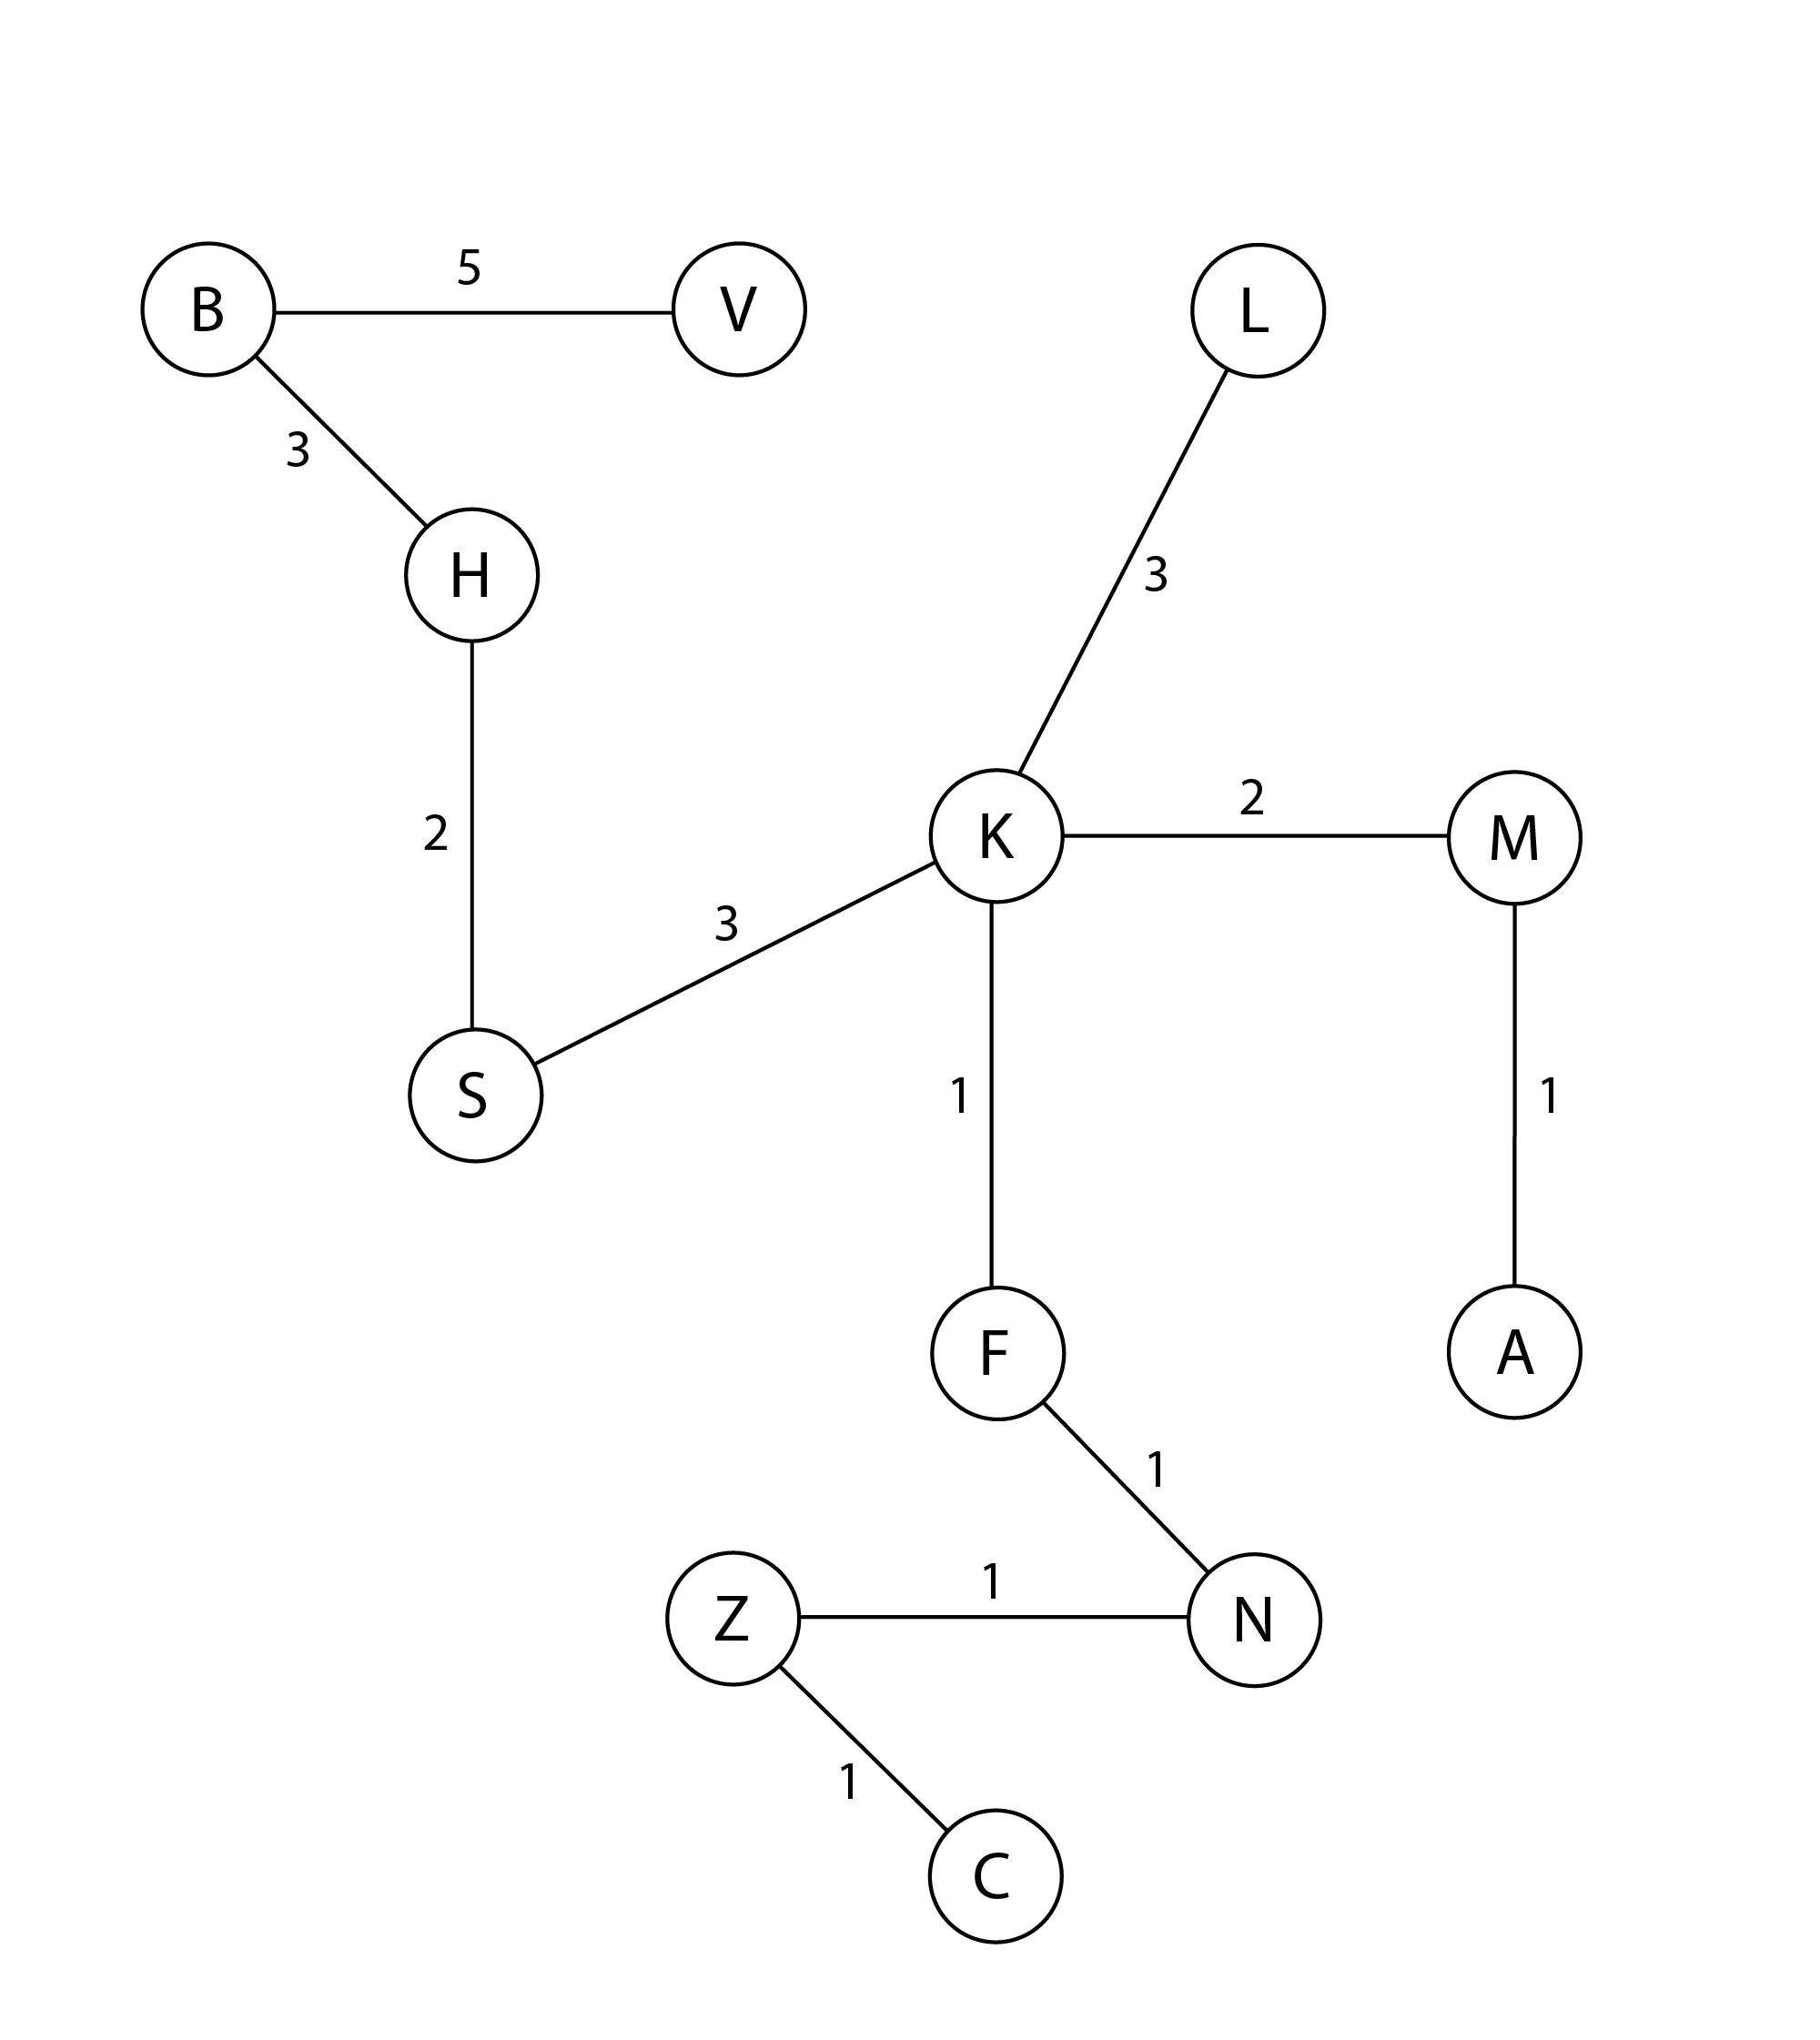
\includegraphics[width=8cm]{prim.png} 
   \caption{Minimaler Spannbaum nach dem Algorithmus von Prim}
   \label{fig:example}
\end{figure}



\subsection*{Ermittlung des minimalen Spannbaum mit dem Algorithmus von Kruskal}

Um den Kruskal Algorithmus anwenden zu können, werden die Kanten zunächst nach Gewicht sortiert:
\begin{table}[h]
   \centering
   \begin{tabular}{@{} ccccccc @{}} % Column formatting, @{} suppresses leading/trailing space
      \toprule
      	Gewicht & Kanten \\
      \midrule
      	1 & ZC, ZN, NF, FK, AM, \\
	2 & ZF, SH, KM, \\
	3 & FA, SK, KL, HB \\
	4 & CN, NA, FS, KH \\
	5 & FM, BV \\
	6 & VH \\
	7 & ML, LV \\
      \bottomrule
   \end{tabular}
   \caption{Sortierung der Kanten nach aufsteigend nach Gewicht (für Kruskal)}
   \label{tab:booktabs}
\end{table}

Die Reihenfolge, in welcher die Kanten dann dem Spannbaum hinzugefügt werden ist nicht eindeutig, da es keine Regel für die Prioritäten von Kanten mit gleichem Gewicht gibt (wir sind im Originalgraph von unten nach oben vorgegangen).

Die Reihenfolge, in der die Kanten in ausgewählt wurden: \\
ZC - ZN - NF - FK - AM - SH - KM - KS - KL - HB - BV \\

Damit ergibt sich eine Summe der Kantengewichte von 23 für den erzeugten Spannbaum.

\begin{figure}[h] %  figure placement: here, top, bottom, or page
   \centering
   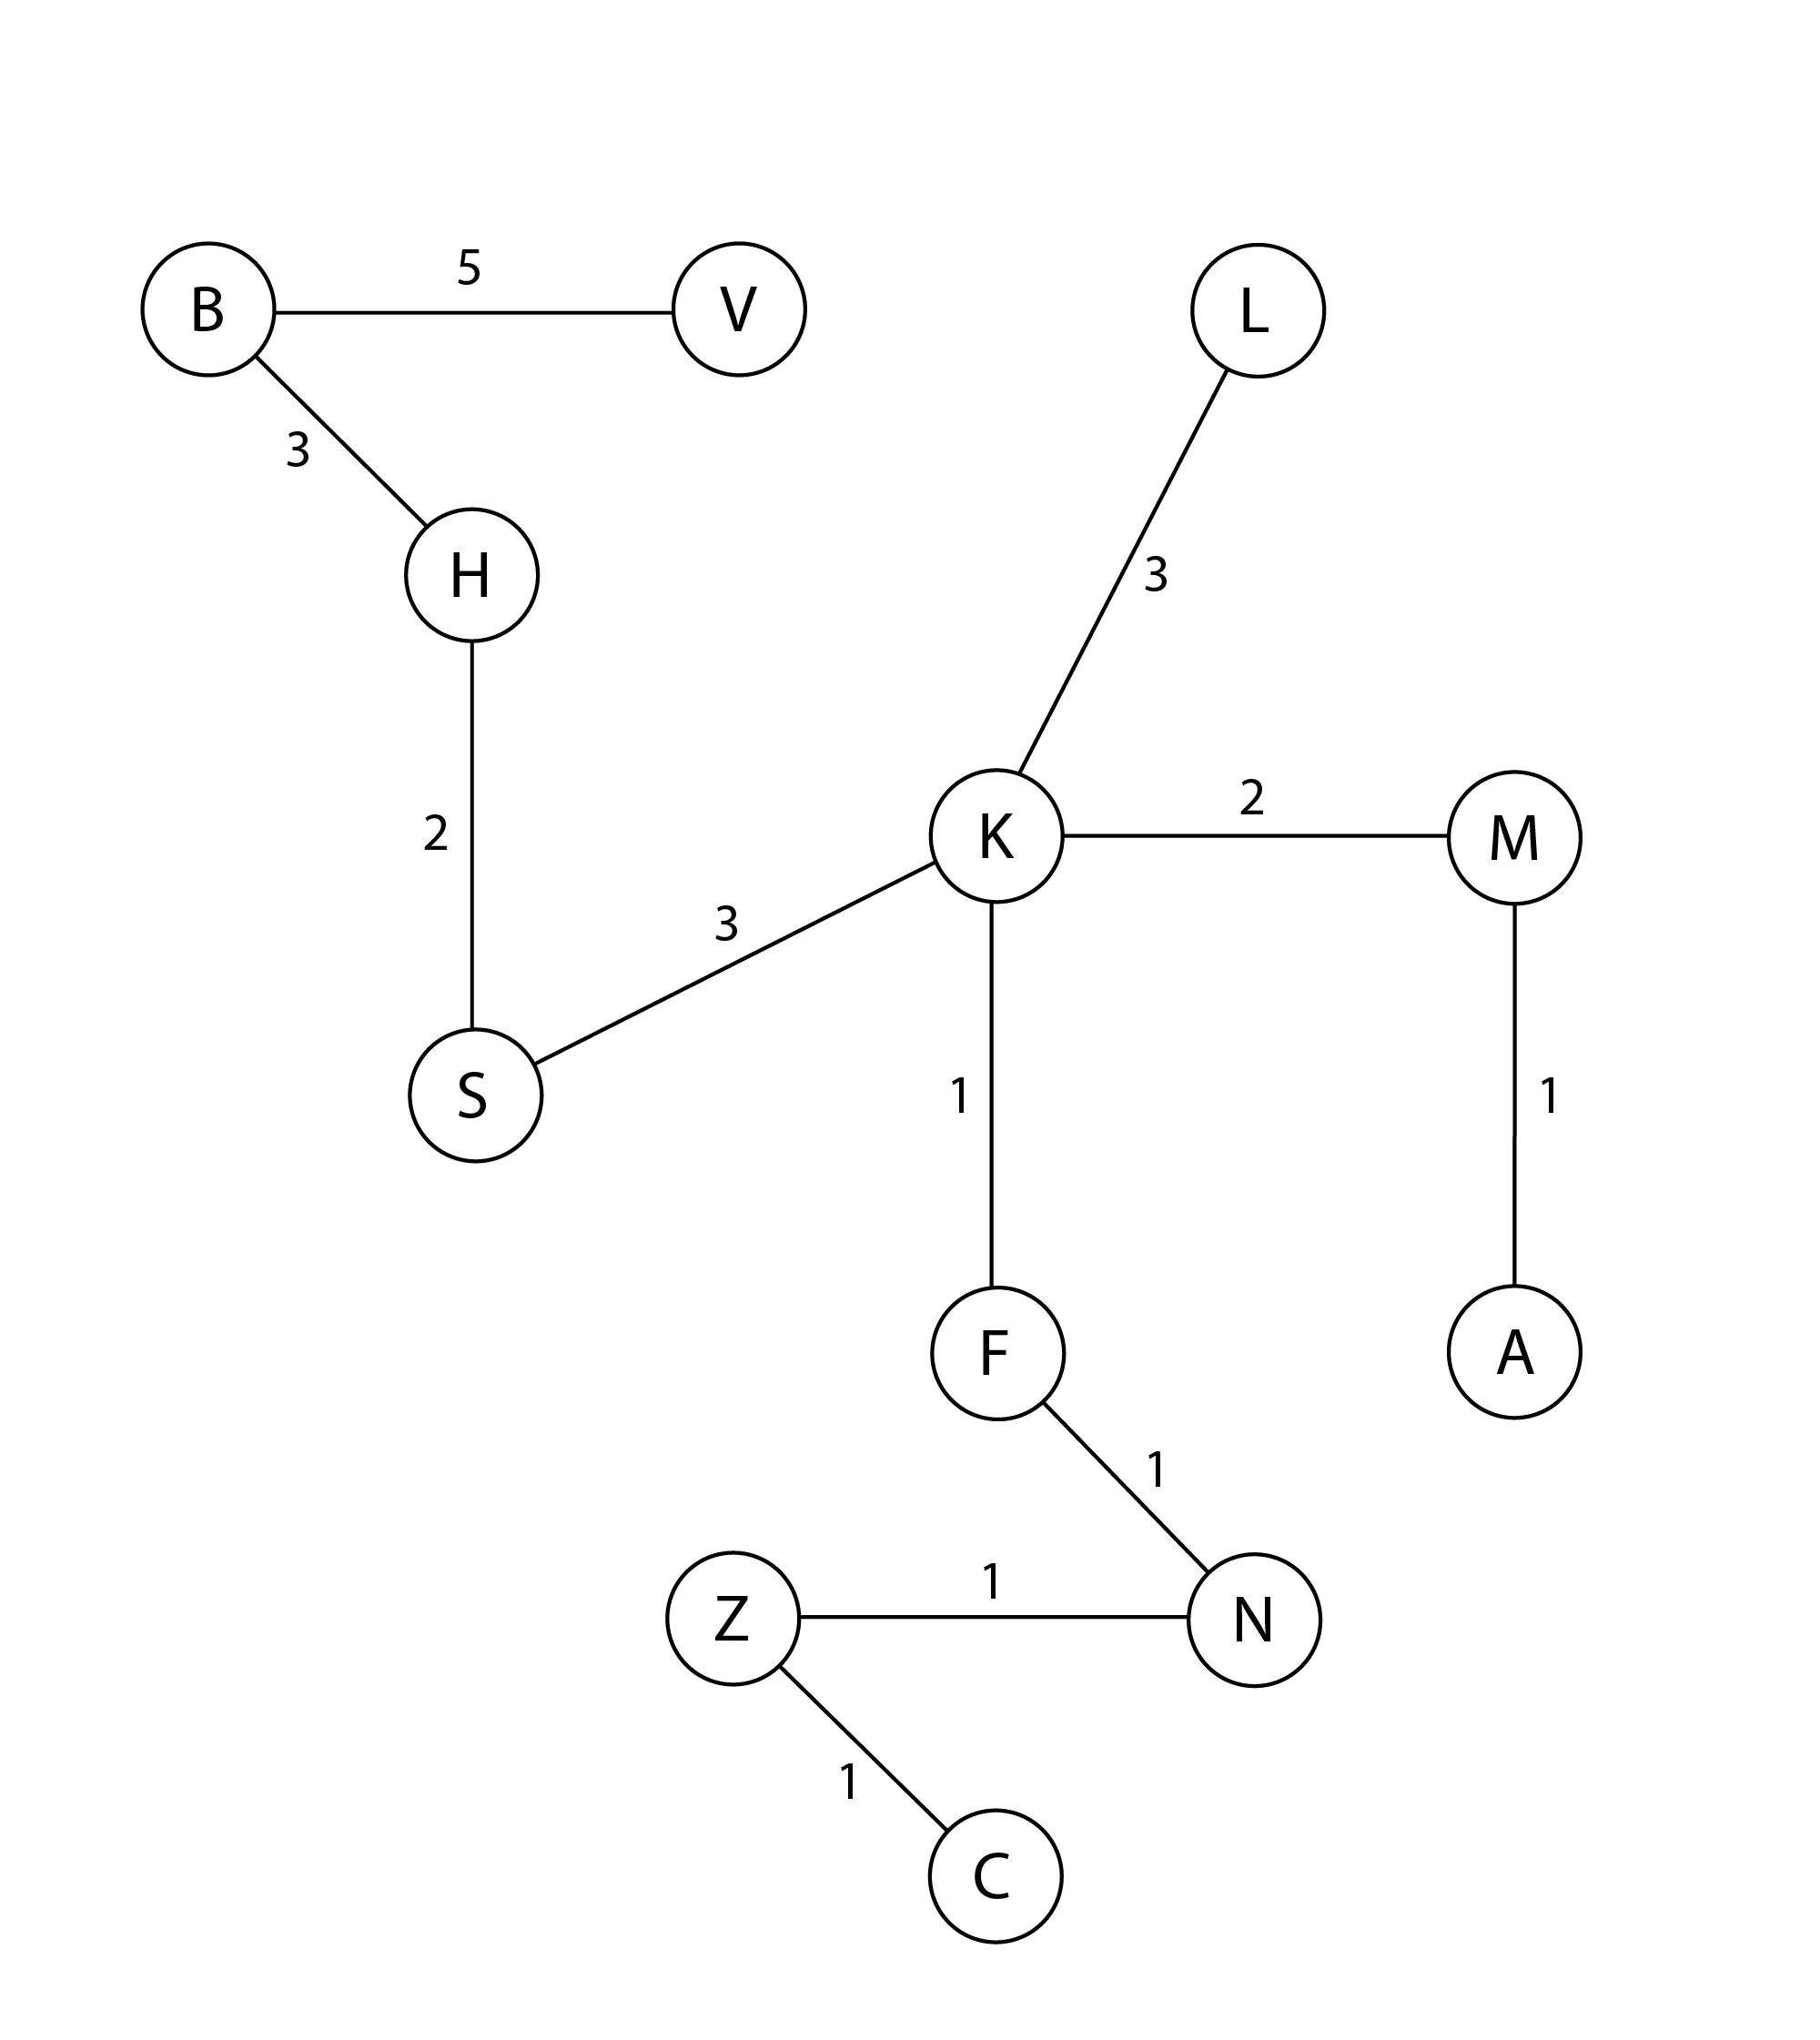
\includegraphics[width=8cm]{prim.png} 
   \caption{Minimaler Spannbaum nach dem Algorithmus von Kruskal}
   \label{fig:example}
\end{figure}

\end{document}